\section{Conclusion}
This paper aimed to determine the optimal design variables for a mechanically interlocking structure of two incompatible materials. 
Two designs were considered, a straight design and a diagonal design. 
After optimizing with a self-implemented SQP algorithm, it was found that the straight interlocking design outperforms the diagonal design.
The maximum stress which can be reached with the straight design is around three times as high as the maximum stress which can be achieved using the diagonal setup.
The design variables $w_b$, $v_a$, $v_b$, $h_f$ and $F$ are equal to 2.68, 2.56, 1.03, 1.20 and 33.91 respectively. 
The tensile strength of the interlocking structure is then 7.36 MPa. 
When comparing this ultimate tensile strength of the interlocking structure to the tensile strength of the weakest of the two materials, Ultimaker PolyPropylene of \SI{10.5}{\mega\pascal}, the tensile strength reaches \SI{70}{\percent} of the base material strength.
This value is relatively high considering the weak chemical bonding between PP and most other thermoplastics.


\subsection{Recommendations}
To account for inaccuracies in the loading conditions, material properties and in manufacturing process, it is recommended to introduce safety factors on a design variables obtained which will slightly increase the obtained optimum.
For the manufacturing, a deposition accuracy of \SI{0.1}{\milli\meter} is a reasonable guesstimate for most desktop FDM 3D printing systems.

The optimum is found at the intersection of several constraint surfaces, each of which has a different gradient at the optimum.
Adding the deposition accuracy to the optimum obtained gives a random perturbation in the design space, the expected stress at the optimum might be lower
compared to a different reference point which is a bit further down along the least steep surface.


Looking at the graphs in \cref{fig:ana_minF} and the sensitivities it makes sense to choose a design with a slightly lower $\hf$ and $\wb$ than the optimum of the straight design.
The sensitivity of $\xvec_i$ in one of the active constraints $\gvec_i$ can then be computed with:
\begin{align*}
	\diffp{f}{{\xvec_i}} + \sum\limits^{j \neq i} \diffp{f}{{\xvec_j}} \left( \diffp{{\gvec_i}}{{\xvec_j}} \right)^{-1} \diffp{{\gvec_i}}{{\xvec_i}}
\end{align*}

In this way, one could compute the expected ultimate strength considering a random perturbation of the design.
However, finding other optimal design parameters given manufacturing inaccuracies falls outside the scope of the current work.

Depending on the application of the interlocking structure, different constraint values might apply.
For other materials the optimum is expected to shift towards another location.
Though the sensitivities show the dependency of the objective function and constraints with respect to the design variables,
deriving the dependency of the actual optimum with respect to the material parameters has not been investigated.
Another important consideration are the values set for the design constraints.
These were chosen based on particular printer limitations, however if these are modified to accomodate for other manufacturing resources the optimum point is expected to shift.
For example, the constraint value $L_{max}$ was varied. \Cref{fig:stress_vs_L} shows that using a bigger design space can achieve higher values for the objective function.

\begin{figure}
	\centering
	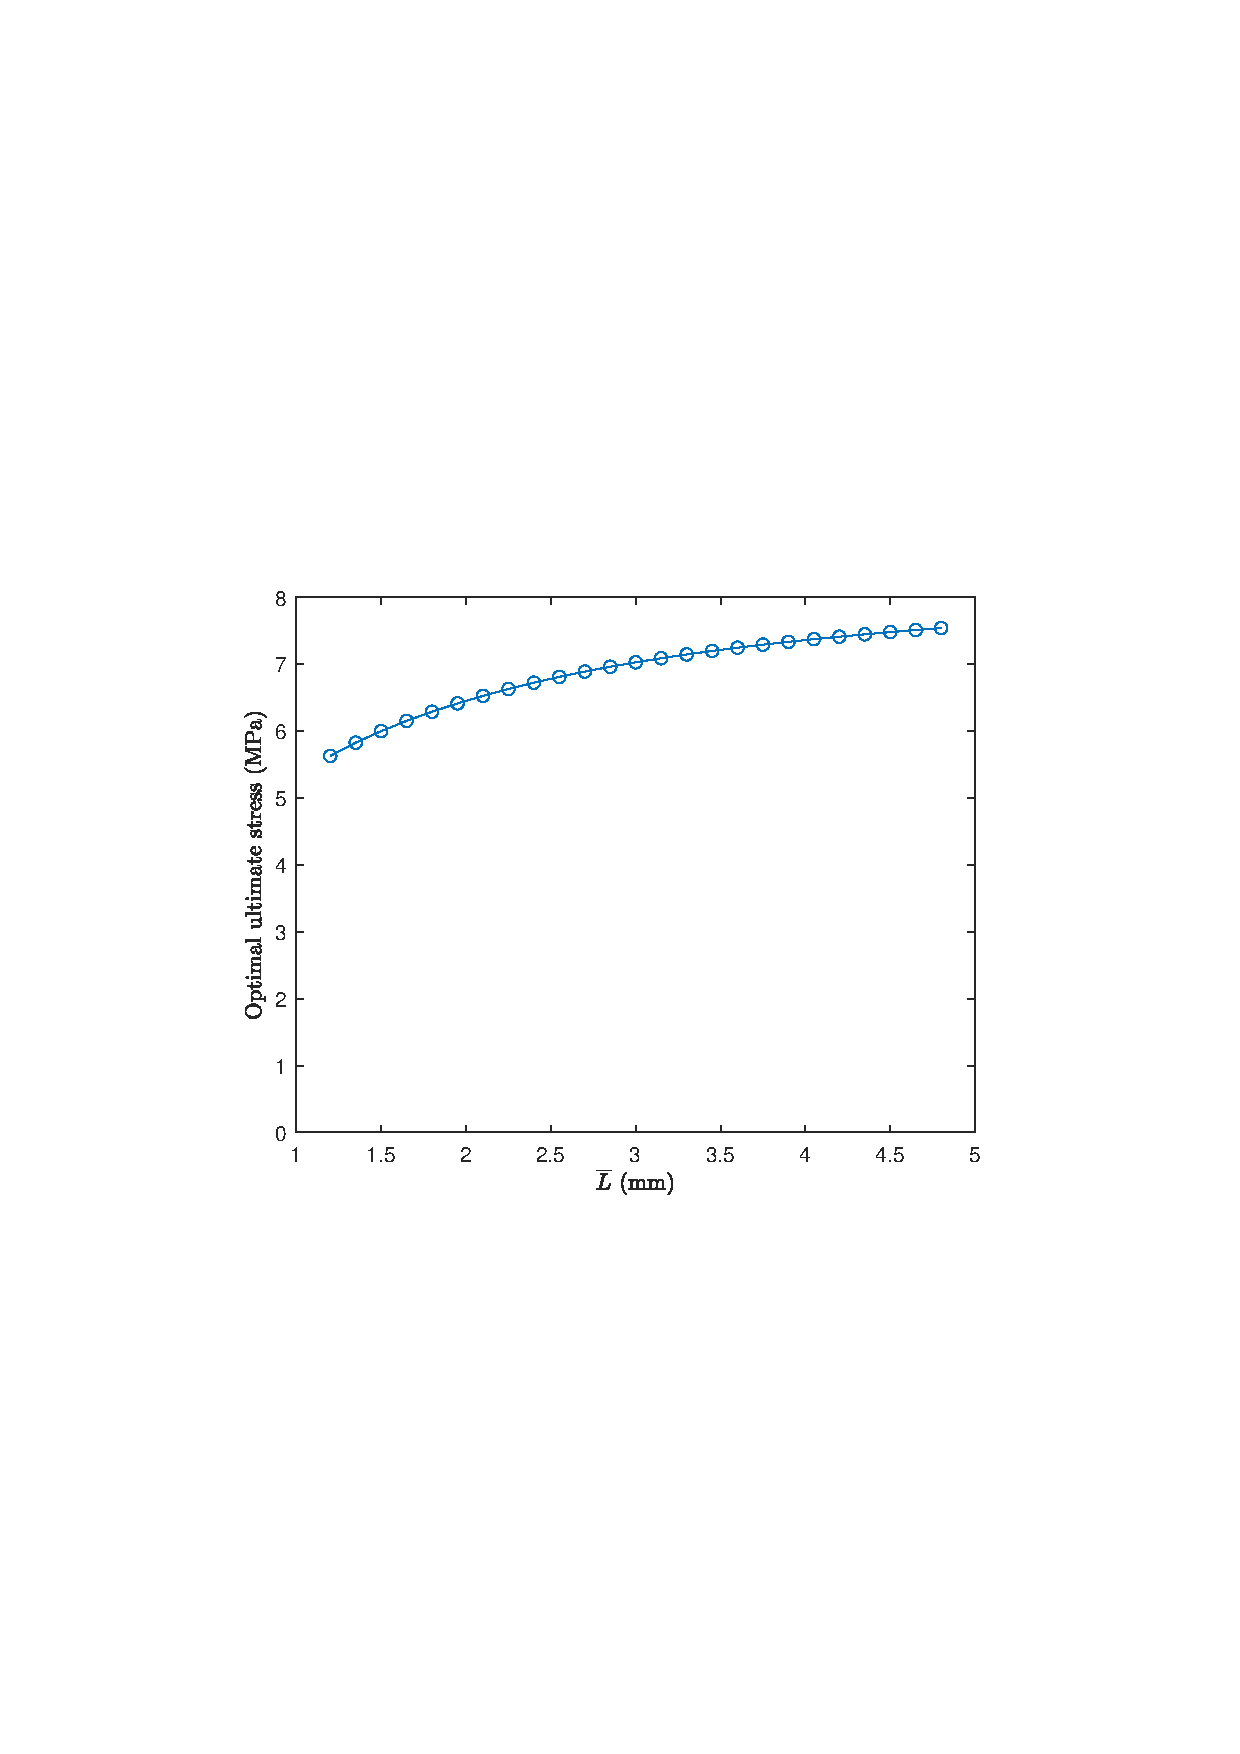
\includegraphics[width=\columnwidth]{sources/method/straight_max_stress_different_L.pdf}
	\caption{The optimal strength for various values of the design constraint $\Lmax$.}
	\label{fig:stress_vs_L}
\end{figure}


\subsection{Limitations and Future work}
In the current optimization problem, the active set and the lambda update strategy require more tuning in order to work for a wider range of design problems
if not with better heuristics then with local iterations to get $\xvec$ and $\lamvec$ closer to their intended values.
Moreover the \texttt{quadprog} encountered problems when updating the design variables for non-convex objective functions, which drove the unconstrained optimization along isolines rather than in the direction of the steepest descent. 

Considering the optimization strategy, also different algorithms can be experienced with. 
For example, if the governing equations are not directly or differentiable, for example when the $max$ out of two variables is taken as suggested, other algorithms like the genetic algorithm, Powell’s Conjugate Directions method or Nelder and Mead Simplex method are recommended to be exploited.

Another limitation is that the manufacturing constraint that $\hf$ should be an integer multiple of $\hmin$ was not accounted for.
SQP doesn't seem to be well suited for the problem at hand, however when looking at the sensitivities it is recommended to round this value up to relax the constraints.

The mathematical problem definition proposed has strong assumptions with respect to the homogeneity of stress distributions throughout the part,
while in reality the disctribution of stress is expected to be heterogenous.
Specifically the validity of the diagonal model is hard to verify, since the angles it hard to analyze the anisotropic behavior.
Also factors such as friction can prove to be significant which has not been accounted for.

One line of future research is directed at different types of interlocking designs.
Does high genus interlocking designs outperform 2D dovetail type interlocking designs for more flexible materials?
How would the optimal interlocking design look for different forces, like shear, or a vertically applied force? These are to be investigated in future research.
